\documentclass[aspectratio=169,10pt]{beamer}

\usetheme{Madrid}
\usecolortheme{seahorse}

\usepackage{amsmath,amssymb}
\usepackage{booktabs}
\usepackage{array}
\usepackage{graphicx}
\usepackage{tikz}
\usetikzlibrary{matrix,positioning,arrows.meta}

% Compact tables
\newcommand{\tmark}{\checkmark}
\setbeamertemplate{navigation symbols}{}
\setbeamertemplate{footline}[frame number]

\title{Measuring Interdisciplinarity:\\
  A Multi-Component Indicator Panel\\
  for Research Evaluation}
\author{A.~Rivero \and A.\,I.~Scaffold}
\date{2026}
\institute{}

\begin{document}

% ======================================================================
% SLIDE 1: Title
% ======================================================================
\begin{frame}
\titlepage
\end{frame}

% ======================================================================
% SLIDE 2: Outline
% ======================================================================
\begin{frame}{Outline}
\tableofcontents
\end{frame}

% ======================================================================
\section{Introduction}
% ======================================================================

% SLIDE 3
\begin{frame}{The Problem}
\begin{itemize}
  \item Interdisciplinary research (IDR) is widely promoted by policy
        initiatives worldwide (National Academies, 2005).
  \item Yet \textbf{measurement remains unsettled}:
  \begin{itemize}
    \item Wang \& Schneider (2020): 23 measures, low mutual correlations
          --- ``no single indicator can unequivocally identify'' IDR.
    \item Leydesdorff et al.\ (2019): Rao-Stirling dominated by disparity,
          limited discriminatory power.
    \item Cantone (2024): IDR is a ``polysemous construct'' ---
          multiple meanings, no single number suffices.
  \end{itemize}
  \item \textbf{Fundamental mismatch}: multidimensional phenomenon
        $\longleftrightarrow$ scalar indicators.
\end{itemize}
\end{frame}

% SLIDE 4
\begin{frame}{This Paper's Contributions}
\begin{enumerate}
  \item \textbf{Taxonomy}: four conceptual dimensions
        $\times$ four methodological families.
  \item \textbf{Panel}: three-component indicator triple $(\Delta, S, E)$
        spanning diversity, coherence, and cross-field effect.
  \item \textbf{Demonstration}: toy data + department-level case study
        show the panel uniquely discriminates integrators, polymaths,
        and specialists.
  \item \textbf{Robustness}: analytical proof that discrimination holds
        under similarity-matrix perturbation.
\end{enumerate}
\end{frame}

% ======================================================================
\section{Conceptual Foundations}
% ======================================================================

% SLIDE 5
\begin{frame}{Stirling's Diversity Framework}
\begin{columns}[T]
\column{0.55\textwidth}
Stirling (2007): diversity requires three properties:
\begin{description}
  \item[Variety] How many categories are represented.
  \item[Balance] How evenly distributed across categories.
  \item[Disparity] How different the categories are from each other.
\end{description}
\medskip
Shannon entropy and Herfindahl capture only variety + balance.

\column{0.42\textwidth}
\textbf{Rao-Stirling index}:
\[
  \Delta = \sum_{i \neq j} d_{ij}\, p_i\, p_j
\]
\begin{itemize}
  \item $p_i$: proportion in category $i$
  \item $d_{ij} = 1 - s_{ij}$: dissimilarity
  \item Incorporates all three properties
\end{itemize}
\end{columns}
\end{frame}

% SLIDE 6
\begin{frame}{Historical Evolution \& Typology}
\begin{itemize}
  \item OECD (1998), Morillo et al.\ (2003) --- tripartite typology:
  \begin{description}
    \item[Multidisciplinary] Juxtaposes perspectives, no synthesis.
    \item[Interdisciplinary] Integrates data, methods, theories ---
          ``greater than the sum of its parts'' (Wagner et al., 2011).
    \item[Transdisciplinary] Transcends disciplinary epistemologies.
  \end{description}
  \item Aksnes et al.\ (2026): 42\% of papers rated as \emph{both}
        multi- and interdisciplinary --- not a clean partition but a spectrum.
  \item Directionality matters: input-side vs.\ output-side IDR
        (Zhou et al., 2023).
\end{itemize}
\end{frame}

% SLIDE 7
\begin{frame}{The Polysemy Problem}
\begin{itemize}
  \item Cantone (2024): IDR is a \textbf{polysemous construct} ---
        physicist + biologist, data scientist, social theorist all called
        ``interdisciplinary.''
  \item Three measurement \emph{approaches} that cluster differently:
  \begin{itemize}
    \item \textbf{Cognitive}: diversity of references, methods, frameworks.
    \item \textbf{Grouping/Social}: co-authorship, affiliations.
    \item \textbf{Semantic}: keywords, abstracts, full-text analysis.
  \end{itemize}
  \item Self-reported $\neq$ bibliometric IDR (Zwanenburg, 2022;
        Aksnes et al., 2026: $r \approx 0.15$).
  \item ``Big'' vs.\ ``small'' interdisciplinarity
        (Morillo et al., 2003).
\end{itemize}
\end{frame}

% SLIDE 8
\begin{frame}{Epistemological \& Validity Challenges}
\begin{itemize}
  \item \textbf{Classification instability}: WoS 254 categories achieve
        only $\sim$50\% alignment with citation-based clusters (Boyack, 2005).
  \item \textbf{Horizontal disciplines}: Nature, Science, PNAS classified
        as ``Multidisciplinary Sciences'' --- low IDR scores despite
        spanning the disciplinary spectrum.
  \item \textbf{Validity crisis} (Zwanenburg et al., 2022):
  \begin{itemize}
    \item Content validity: indicators capture only 1--2 of 3 diversity properties.
    \item Domain validity: ambiguous journal-to-category mappings.
    \item Coherence validity: notionally equivalent measures diverge.
  \end{itemize}
  \item Rafols (2019): responsible metrics need both analytical validity
        \emph{and} social robustness.
\end{itemize}
\end{frame}

% ======================================================================
\section{Taxonomy of Indicators}
% ======================================================================

% SLIDE 9
\begin{frame}{Taxonomy Overview}
\small
\begin{table}
\centering
\begin{tabular}{@{}l p{2.9cm} p{2.9cm} p{2.2cm} p{2.5cm}@{}}
\toprule
\textbf{Dimension} & \textbf{Reference-based} & \textbf{Citation-based}
  & \textbf{Text-based} & \textbf{Network-based} \\
\midrule
Diversity  & Rao-Stirling, Simpson, Shannon, Gini, Hill & --- & Semantic similarity & --- \\
Coherence  & Bibliographic coupling density & --- & --- & Betweenness, clustering \\
Diffusion  & --- & Cross-field cites, citing diversity & --- & --- \\
Novelty    & --- & --- & --- & Recombination metrics \\
\bottomrule
\end{tabular}
\end{table}
\medskip
\begin{itemize}
  \item Reference-based/diversity cell is heavily populated; others sparse.
  \item Coherence and diffusion are orthogonal to diversity (Wang \& Schneider, 2020).
  \item No existing indicator spans multiple dimensions $\Rightarrow$
        need a multi-component panel.
\end{itemize}
\end{frame}

% SLIDE 10
\begin{frame}{Diversity Indicators: Key Results}
\begin{itemize}
  \item \textbf{Variety + Balance only}: Shannon $H$, Simpson $D_\mathrm{Sim}$,
        Brillouin, Gini --- intercorrelate $r \in [0.60, 1.00]$, but only
        weakly with disparity measures.
  \item \textbf{Rao-Stirling} $\Delta = \sum_{i\neq j} d_{ij}\,p_i\,p_j$:
        most widely used, but highly sensitive to $s_{ij}$ specification.
  \item Wang \& Schneider (2020): 8 RS variants; pairwise $r$ as low as 0.18.
  \item \textbf{Hill-type true diversity} (Zhang et al., 2016):
  \[
    {}^2D^S = \frac{1}{\sum_{i,j} s_{ij}\,p_i\,p_j} = \frac{1}{1-\Delta}
  \]
  Interpretation as ``effective number of disciplines'';
  satisfies replication principle.
  \item \textbf{Similarity matrix}: construction (Salton vs.\ Ochiai cosine)
        is a first-order determinant of results.
\end{itemize}
\end{frame}

% SLIDE 11
\begin{frame}{Validity Assessment (Zwanenburg et al., 2022)}
21 measures evaluated against 8 criteria:
\begin{enumerate}\small
  \item \textbf{Applicability}: (a) Multi-object, (b) Size independence.
  \item \textbf{Integration evidence}: measure should reflect actual
        knowledge integration.
  \item \textbf{Discipline identification}: (a) Valid allocation,
        (b) Completeness, (c) Low classification bias.
  \item \textbf{Diversity capture}: (a) Sensitivity to variety + balance + disparity,
        (b) Decomposability.
\end{enumerate}
\medskip
\begin{itemize}
  \item Only 6 of 21 met criterion 2 (integration evidence).
  \item \textbf{No single measure} satisfied all 8 criteria.
  \item $\sim$30\% of references assigned to multiple WoS categories
        $\Rightarrow$ allocation ambiguity cascades into inflated scores.
\end{itemize}
\end{frame}

% SLIDE 12
\begin{frame}{Coherence Indicators}
\begin{columns}[T]
\column{0.55\textwidth}
\textbf{Key idea} (Rafols \& Meyer, 2009): do diverse inputs form a
unified intellectual fabric, or are they merely juxtaposed?
\medskip
\textbf{Mean linkage strength}:
\[
  S = \frac{2}{N(N-1)} \sum_{a < b} s_{ab}
\]
where $s_{ab} = \cos(\mathbf{r}_a, \mathbf{r}_b)$ via
bibliographic coupling.

\column{0.42\textwidth}
\textbf{Diversity--Coherence matrix}:
\medskip
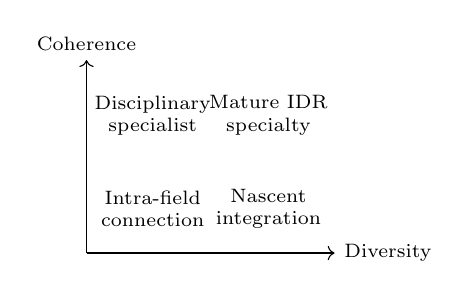
\begin{tikzpicture}[scale=0.7, every node/.style={font=\scriptsize}]
  \draw[->] (0,0) -- (4.5,0) node[right]{Diversity};
  \draw[->] (0,0) -- (0,3.5) node[above]{Coherence};
  \node[align=center] at (1.2,2.5) {Disciplinary\\specialist};
  \node[align=center] at (3.3,2.5) {Mature IDR\\specialty};
  \node[align=center] at (1.2,0.8) {Intra-field\\connection};
  \node[align=center] at (3.3,0.8) {Nascent\\integration};
\end{tikzpicture}
\end{columns}
\medskip
\begin{itemize}
  \item Empirically orthogonal to diversity ($r < 0.5$; Wang \& Schneider, 2020).
  \item Captures depth of integration, not breadth.
\end{itemize}
\end{frame}

% SLIDE 13
\begin{frame}{Diffusion Indicators}
\begin{itemize}
  \item Look \textbf{forward}: who cites the work across fields?
  \item Replace reference vector $\mathbf{p}(x)$ with citation vector
        $\mathbf{q}(x)$.
  \item Leydesdorff et al.\ (2019) --- \textbf{DIV indicator}:
  \[
    \mathrm{DIV}_c = \frac{n_c}{N}\;(1 - G_c)\;
    \frac{\sum_{i\neq j} d_{ij}}{n_c(n_c-1)}
  \]
  monotonically increasing in each component.
  \item Highest-scoring journals: \emph{PLOS ONE}, \emph{Science}, \emph{Nature}.
  \item Xiang et al.\ (2025): knowledge-base IDR $\uparrow$ acceptance;
        topic IDR $\downarrow$ acceptance.
  \item \textbf{Conceptual tension}: diffusion is an \emph{outcome},
        not a property of the research process (Cantone, 2024).
\end{itemize}
\end{frame}

% SLIDE 14
\begin{frame}{Novelty Indicators}
\begin{itemize}
  \item Is a combination \textbf{atypical}, not just diverse?
  \item \textbf{Uzzi et al.\ (2013)}: z-score against permuted citation
        networks.
  \item \textbf{Wang et al.\ (2017)}: timed novelty --- weight by recency
        of first combination.
  \item \textbf{Validation failures}:
  \begin{itemize}
    \item Bornmann (2019): no correlation with F1000Prime expert assessments.
    \item Fontana et al.\ (2020): Uzzi measure correlates with
          Rao-Stirling diversity instead.
  \end{itemize}
  \item[$\Rightarrow$] \textbf{Excluded from our panel}: high data
        requirements + failed external validation.
  \item Novelty remains an important \emph{conceptual} dimension;
        awaits better operationalization.
\end{itemize}
\end{frame}

% ======================================================================
\section{The Multi-Component Panel}
% ======================================================================

% SLIDE 15
\begin{frame}{Panel Definition: $(\Delta, S, E)$}
\begin{description}
  \item[Diversity $\Delta$] Rao-Stirling index over aggregate reference
        proportions:
  \[
    \Delta = 1 - \sum_{i,j} s_{ij}\, p_i\, p_j
  \]
  \item[Coherence $S$] Mean bibliographic-coupling cosine across
        publication pairs:
  \[
    S = \frac{1}{\binom{n}{2}} \sum_{k<l}
    \cos(\mathbf{r}_k, \mathbf{r}_l)
  \]
  \item[Cross-field effect $E$] Fraction of citations from outside
        each publication's primary category:
  \[
    E = \frac{\text{cross-field citations}}{\text{total citations}}
  \]
\end{description}
\medskip
Each component captures an \textbf{independent} dimension;
only $\Delta$ depends on the similarity matrix $\mathbf{S}$.
\end{frame}

% SLIDE 16
\begin{frame}{Toy Data: Setup}
Five categories; three researcher archetypes:
\medskip
\small
\begin{columns}[T]
\column{0.48\textwidth}
\textbf{Similarity matrix}:
\[
\mathbf{S} =
\begin{pmatrix}
1.00 & 0.60 & 0.40 & 0.10 & 0.30\\
0.60 & 1.00 & 0.50 & 0.15 & 0.20\\
0.40 & 0.50 & 1.00 & 0.35 & 0.10\\
0.10 & 0.15 & 0.35 & 1.00 & 0.05\\
0.30 & 0.20 & 0.10 & 0.05 & 1.00
\end{pmatrix}
\]

\column{0.48\textwidth}
\textbf{Researcher profiles}:
\begin{itemize}\footnotesize
  \item \textbf{A} (Integrator): each paper references
        multiple distant categories.\\
        $\mathbf{p}_A = (0.30, 0.08, 0.18, 0.35, 0.10)$
  \item \textbf{B} (Polymath): 5 single-field papers, one per category.\\
        $\mathbf{p}_B = (0.20, 0.20, 0.20, 0.20, 0.20)$
  \item \textbf{C} (Specialist): all papers in condensed matter + materials.\\
        $\mathbf{p}_C = (0.64, 0.27, 0.06, 0.00, 0.03)$
\end{itemize}
\end{columns}
\end{frame}

% SLIDE 17
\begin{frame}{Toy Data: Results --- Single Indicators Fail}
\begin{table}
\centering
\begin{tabular}{@{}l ccc l@{}}
\toprule
\textbf{Researcher} & $\Delta$ & $S$ & $E$ & \textbf{Type} \\
\midrule
A (integrator)   & 0.559 & 0.733 & 0.600 & Cross-disciplinary \\
B (polymath)     & 0.580 & 0.000 & 0.063 & Polymathic breadth \\
C (specialist)   & 0.245 & 0.881 & 0.211 & Disciplinary \\
\bottomrule
\end{tabular}
\end{table}
\bigskip
\textbf{Key finding}: $\Delta_A \approx \Delta_B$ (0.559 vs.\ 0.580).
\begin{itemize}
  \item Diversity \emph{alone} cannot distinguish integrator from polymath.
  \item $S$ reveals the difference: $S_A = 0.73$ (shared references)
        vs.\ $S_B = 0.00$ (orthogonal publications).
  \item $E$ confirms at impact level: $E_A = 0.60$ vs.\ $E_B = 0.06$.
  \item \textbf{Only the full triple uniquely characterizes each type.}
\end{itemize}
\end{frame}

% SLIDE 18
\begin{frame}{Sensitivity Analysis: Robustness Guarantees}
\textbf{Proposition} (uniform perturbation $s_{ij} \to s_{ij} + \varepsilon$):
\[
  \Delta_\mathrm{new} = \Delta_\mathrm{old} - \varepsilon\,(1 - H)
  \qquad\text{where } H = \textstyle\sum_i p_i^2.
\]
\textbf{Corollary}: ranking inverts at critical perturbation
\[
  \varepsilon^* = -\frac{\Delta_A - \Delta_B}{H_A - H_B} = 0.351
\]
--- requires shifting \emph{every} similarity by $>$35\%.

\medskip
\begin{itemize}
  \item Non-uniform perturbation experiments confirm robustness
        under realistic scenarios.
  \item \textbf{Crucially}: $S$ and $E$ are \emph{exactly invariant}
        under any similarity-matrix perturbation.
  \item $\Rightarrow$ Panel discrimination is substantially more robust
        than any single-indicator approach.
\end{itemize}
\end{frame}

% SLIDE 19
\begin{frame}{Interpretation Framework: Pattern Taxonomy}
\begin{table}
\centering\small
\begin{tabular}{@{}l ccc l@{}}
\toprule
\textbf{Pattern} & $\Delta$ & $S$ & $E$ & \textbf{Interpretation} \\
\midrule
Genuine integrator     & High & High & High & Cross-disciplinary synthesis \\
Polymath               & High & Low  & Low  & Breadth without integration \\
Specialist             & Low  & High & Low  & Narrow disciplinary focus \\
Emergent / sparse data & Low  & Low  & Any  & Defer to expert review \\
\bottomrule
\end{tabular}
\end{table}
\bigskip
\textbf{Illustrative thresholds} for operational deployment:
\begin{table}
\centering\small
\begin{tabular}{@{}l ccc@{}}
\toprule
\textbf{Classification} & $\Delta$ & $S$ & $E$ \\
\midrule
Genuine integrator           & $\geq 0.40$ & $\geq 0.30$ & $\geq 0.30$ \\
Polymath (non-integrative)   & $\geq 0.40$ & $< 0.15$    & $< 0.15$ \\
Specialist (reclassify)      & $< 0.35$    & any          & any \\
Ambiguous (expert review)    & else         & else         & else \\
\bottomrule
\end{tabular}
\end{table}
\end{frame}

% SLIDE 20
\begin{frame}{Edge Cases and Failure Modes}
\begin{enumerate}\small
  \item \textbf{Breadth-without-depth}: High $\Delta$ without integration.\\
        \emph{Mitigation}: require $S$ and $E$ thresholds.
  \item \textbf{Non-standard publication penalty}: IDR journals often have
        lower impact factors.\\
        \emph{Mitigation}: field-normalized citation indicators.
  \item \textbf{Incommensurable citation norms}: citation rates differ
        across fields by an order of magnitude.\\
        \emph{Mitigation}: normalize $E$ by field baselines.
  \item \textbf{Misclassification persistence}: specialist stays on IDR
        track.\\
        \emph{Mitigation}: automatic reclassification trigger ($\Delta < 0.35$).
  \item \textbf{Early-career data sparsity}: $< 15$ publications
        $\Rightarrow$ unstable estimates.\\
        \emph{Mitigation}: minimum publication threshold + confidence intervals.
  \item \textbf{Gaming via strategic co-authorship}: inflates $\Delta$
        without integration.\\
        \emph{Mitigation}: cross-check against $S$.
\end{enumerate}
\end{frame}

% ======================================================================
\section{Measurement in Practice}
% ======================================================================

% SLIDE 21
\begin{frame}{Practical Implementation Pipeline}
Cantone (2024) --- five-step pipeline:
\begin{enumerate}
  \item \textbf{Unit of analysis}: paper, author, institution, journal.
  \item \textbf{Taxonomy}: WoS (254 categories), OECD (40), OpenAlex.
  \item \textbf{Classification method}: journal-based, reference-based,
        semantic (LLM), collaboration-based.
  \item \textbf{Operational definition}: dimension + formula selection.
  \item \textbf{Aggregation}: elementary (per-paper mean) vs.\
        collective (pooled references).
\end{enumerate}
\medskip
\textbf{Key finding}: measures cluster by method, not by dimension
(Cantone, 2024).\\
\textbf{Implication}: document every methodological choice explicitly.
\end{frame}

% SLIDE 22
\begin{frame}{Institutional \& National Deployment}
\begin{columns}[T]
\column{0.48\textwidth}
\textbf{Institutional self-assessment}:
\begin{itemize}
  \item $\Delta$ and $S$ computable from internal data.
  \item $E$ requires external citation data (WoS, Scopus, OpenAlex).
  \item Two-component profile $(\Delta, S)$ still discriminates
        integrators from polymaths.
\end{itemize}

\column{0.48\textwidth}
\textbf{National agencies}:
\begin{itemize}
  \item Spain's CNEAI --- \textbf{Campo 0}: first dedicated IDR
        evaluation track (2023).
  \item Criteria map onto panel:
  \begin{itemize}\footnotesize
    \item ``Interdisciplinar'' $\leftrightarrow$ high $\Delta$ + high $S$.
    \item ``Multidisciplinar'' $\leftrightarrow$ high variety $N \geq 2$.
  \end{itemize}
  \item Transdisciplinary: absent from criteria ---
        no standard bibliometric indicator exists.
\end{itemize}
\end{columns}
\end{frame}

% ======================================================================
\section{Open Problems}
% ======================================================================

% SLIDE 23
\begin{frame}{Open Problems (I)}
\begin{enumerate}
  \item \textbf{Self-reported vs.\ bibliometric IDR}: correlations
        only $r \approx 0.15$ (Aksnes et al., 2026). Researchers assess IDR
        via collaboration and methods, not reference patterns.
  \item \textbf{LLM-based similarity matrices}: Cantone (2025) shows
        partial agreement with citation-based estimates; could
        democratize access to disparity-sensitive IDR measurement.
  \item \textbf{Uncertainty quantification}: Nakhoda et al.\ (2023)
        --- bootstrap 95\% CIs span up to 0.6 for Rao-Stirling.
        Point estimates can be misleading.
  \item \textbf{IDR and quality}: short-term citation penalty for IDR
        (Lariviere \& Gingras, 2010), but longer horizons show greater
        lasting impact. Direction matters: knowledge-base IDR $\uparrow$
        acceptance, topic IDR $\downarrow$ (Xiang et al., 2025).
\end{enumerate}
\end{frame}

% SLIDE 24
\begin{frame}{Open Problems (II)}
\begin{enumerate}\setcounter{enumi}{4}
  \item \textbf{Distribution-based approaches}: Zhou et al.\ (2023)
        IKF framework $(B, I, H)$ decomposes what Rao-Stirling aggregates.
  \item \textbf{Participatory indicators}: Marres \& de Rijcke (2020)
        --- ``engaging indicators'' that combine scientometrics with
        stakeholder workshops. Challenge: scaling to national level.
  \item \textbf{Transdisciplinary measurement}: no standard bibliometric
        indicator captures engagement with non-academic partners
        (Borlaug \& Svartefoss, 2025). Spain's Campo 0 omits it entirely.
\end{enumerate}
\end{frame}

% ======================================================================
\section{Case Study}
% ======================================================================

% SLIDE 25
\begin{frame}{Department-Level Case Study: Setup}
Hypothetical Physics \& Materials Science department, 7 researchers.\\
Six WoS categories ($C_1$--$C_6$): condensed matter, materials science,
physical chemistry, optics, electrical engineering, nanoscience.
\medskip
\begin{table}
\centering\scriptsize
\begin{tabular}{@{}l c c l c c@{}}
\toprule
\textbf{Researcher} & \textbf{Stage} & \textbf{Pubs}
  & $\mathbf{p}=(p_1,\ldots,p_6)$ & \textbf{Cites} & \textbf{Cross-field} \\
\midrule
Chen      & S & 42 & (0.35, 0.30, 0.20, 0.05, 0.05, 0.05) & 520 & 35\% \\
Al-Rahman & M & 35 & (0.20, 0.20, 0.20, 0.20, 0.15, 0.05) & 280 & 11\% \\
Kowalski  & E & 18 & (0.65, 0.25, 0.06, 0.02, 0.01, 0.01) &  85 & 12\% \\
Nguyen    & S & 55 & (0.25, 0.25, 0.15, 0.10, 0.15, 0.10) & 890 & 47\% \\
Romero    & M & 28 & (0.10, 0.15, 0.05, 0.05, 0.10, 0.55) & 195 & 72\% \\
Karlsson  & E & 12 & (0.50, 0.30, 0.10, 0.05, 0.03, 0.02) &  45 & 18\% \\
Osei      & S & 48 & (0.70, 0.20, 0.05, 0.03, 0.01, 0.01) & 680 & 11\% \\
\bottomrule
\end{tabular}
\end{table}
\end{frame}

% SLIDE 26
\begin{frame}{Case Study: Panel Results}
\begin{table}
\centering
\begin{tabular}{@{}l ccc l@{}}
\toprule
\textbf{Researcher} & $\Delta$ & $S$ & $E$ & \textbf{Classification} \\
\midrule
Chen      & 0.390 & 0.42 & 0.35 & Moderate integrator \\
Al-Rahman & 0.610 & 0.04 & 0.11 & \textcolor{red}{Polymath} \\
Kowalski  & 0.190 & 0.53 & 0.12 & Specialist \\
Nguyen    & 0.464 & 0.50 & 0.47 & \textcolor{teal}{Strong integrator} \\
Romero    & 0.374 & 0.50 & 0.72 & Niche-bridge specialist \\
Karlsson  & 0.244 & 0.58 & 0.18 & Early-career specialist \\
Osei      & 0.176 & 0.58 & 0.11 & Specialist \\
\bottomrule
\end{tabular}
\end{table}
\medskip
\begin{itemize}
  \item \textbf{Al-Rahman}: highest $\Delta$ in department, but $S \approx 0$
        and $E = 0.11$ $\Rightarrow$ polymath, \emph{not} integrator.
  \item \textbf{Romero}: moderate $\Delta$ but exceptional $E = 0.72$
        $\Rightarrow$ bridge-specialist requiring expert review.
  \item \textbf{Nguyen}: exceeds all three thresholds $\Rightarrow$
        genuine integrator.
\end{itemize}
\end{frame}

% SLIDE 27
\begin{frame}{Case Study: Single Indicators Compared}
\begin{table}
\centering\small
\begin{tabular}{@{}l l l l@{}}
\toprule
\textbf{Rank} & \textbf{Shannon $H$} & \textbf{Rao-Stirling $\Delta$}
  & \textbf{Cross-field $E$} \\
\midrule
1 & Al-Rahman (2.43) & Al-Rahman (0.610) & Romero (0.72) \\
2 & Nguyen (2.32) & Nguyen (0.464) & Nguyen (0.47) \\
3 & Chen (2.05) & Chen (0.390) & Chen (0.35) \\
\bottomrule
\end{tabular}
\end{table}
\bigskip
\begin{itemize}
  \item Each single indicator produces a \textbf{different} ``most interdisciplinary''
        researcher.
  \item Shannon and RS both rank the polymath \#1.
  \item Cross-field effect ranks the bridge specialist \#1.
  \item \textbf{Full panel avoids all three errors}:
        Al-Rahman's zero coherence unmasks the polymath;
        Romero is flagged for expert review;
        Nguyen is confirmed as genuine integrator.
\end{itemize}
\end{frame}

% ======================================================================
\section{Conclusions}
% ======================================================================

% SLIDE 28
\begin{frame}{Conclusions}
\begin{enumerate}
  \item \textbf{No single indicator is adequate} for measuring IDR.
        The literature is heavily concentrated on diversity;
        coherence, diffusion, and novelty are underexplored.
  \item The \textbf{three-component panel} $(\Delta, S, E)$:
  \begin{itemize}
    \item Spans three orthogonal dimensions.
    \item Uniquely discriminates integrators, polymaths, and specialists.
    \item Robust under similarity-matrix perturbation ($\varepsilon^* = 0.35$).
    \item $S$ and $E$ are exactly invariant to the similarity matrix.
  \end{itemize}
  \item \textbf{Practical implications}:
  \begin{itemize}
    \item Evaluation agencies should use multidimensional profiles,
          not composite scores.
    \item Thresholds must be calibrated to local context.
    \item Report confidence intervals + methodological specifications.
  \end{itemize}
  \item \textbf{Next steps}: empirical validation on real university data;
        integration of LLM-based similarity; uncertainty quantification.
\end{enumerate}
\end{frame}

% ======================================================================
% SLIDE 29: Thank you / Questions
% ======================================================================
\begin{frame}{}
\vfill
\centering
{\Huge Thank you}

\bigskip
{\large Questions?}

\bigskip
\texttt{arivero@unizar.es}
\vfill
\end{frame}

% ======================================================================
% SLIDE 30: Selected References
% ======================================================================
\begin{frame}[allowframebreaks]{Selected References}
\scriptsize
\begin{itemize}
  \item Cantone (2024). How to measure IDR? A systemic design.
        \emph{Scientometrics}, 129:4937--4982.
  \item Leydesdorff, Wagner, Bornmann (2019). IDR as diversity in
        citation patterns. \emph{J.\ Informetrics}, 13:255--269.
  \item Morillo, Bordons, G\'omez (2003). IDR typology of disciplines.
        \emph{JASIST}, 54:1237--1249.
  \item Nakhoda, Whigham, Zwanenburg (2023). Uncertainty in IDR
        measurement. \emph{Scientometrics}, 128:6107--6127.
  \item Porter, Rafols (2009). Is science becoming more interdisciplinary?
        \emph{Scientometrics}, 81:719--745.
  \item Rafols (2019). S\&T indicators in the wild.
        \emph{Research Evaluation}, 28:7--22.
  \item Rafols, Meyer (2009). Diversity and coherence in bionanoscience.
        \emph{Scientometrics}, 82:263--287.
  \item Stirling (2007). Framework for analysing diversity.
        \emph{J.\ R.\ Soc.\ Interface}, 4:707--719.
  \item Wang, Schneider (2020). Consistency and validity of IDR measures.
        \emph{QSS}, 1:239--263.
  \item Xiang, Romero, Teplitskiy (2025). Evaluating IDR: topic vs.\
        knowledge base. \emph{PNAS}, 122:e2409752122.
  \item Zhang, Rousseau, Gl\"anzel (2016). Diversity of references
        as IDR indicator. \emph{JASIST}, 67:1257--1265.
  \item Zhou, Guns, Engels (2023). Characterizing interdisciplinary
        knowledge flow. \emph{JASIST}, 74:1325--1340.
  \item Zwanenburg, Nakhoda, Whigham (2022). Consistency and validity
        evaluation. \emph{Scientometrics}, 127:3035--3065.
\end{itemize}
\end{frame}

\end{document}
